%%%%%%%%%%%%%%%%%%%%%%%%%%%%%%%%%%%%%%%%%%%%%%%%%%%%%%%%%%%%%%%%%
\chapter{CONCLUSION AND FUTURE WORK}\label{Ch6}
%%%%%%%%%%%%%%%%%%%%%%%%%%%%%%%%%%%%%%%%%%%%%%%%%%%%%%%%%%%%%%%%%

In this study a compact RF ion thruster system was designed for cube satellite applications. Limitations emposed by cube satellite standards were briefly mentioned and literature research regarding the current state of the RF ion thruster technology was presented. Working principle of an RF ion thruster were explained. A detailed design study was then performed on the RF ion thruster. Limitations emposed by the cube satellite standards were given. Based on the design parameters calculations were performed to determine the amount of thrust and specific impulse the thruster can generate. 

A series of firing tests were then conducted in a vacuum chamber. Details about the experimental setup and environment were provided. Initial tests had resulted in failure due to mechanical complications within the ion accelerator grids of the thruster. These mechanical complications included the low production quality of the grids, imperfections and burrs left behind after laser cutting process. First three tests had resulted in an electrical short forming between grids and thus had failed. Material and production process of the grids were then changed. Eventually on the fourth test the thruster was operated as intended. 

Not all of research objectives were met. During experiments the thruster was observed to accelerate ions in the form of ion beamlets which is a visual indication of thrust generation. However due to lack of experimental setup no results regarding ion beam characteristics were recorded. A faraday probe, or cup, would be used to record the ion beam charge. Various types of faraday probes have been used in the studies electic propulsion systems to determine ion beam characteristics.


For this study a guardad planar type of faraday probe would be used. An exploded CAD view of the probe is provided in figure \ref{fig:explodedfaraday}.


\begin{figure}[ht]
    \centering
    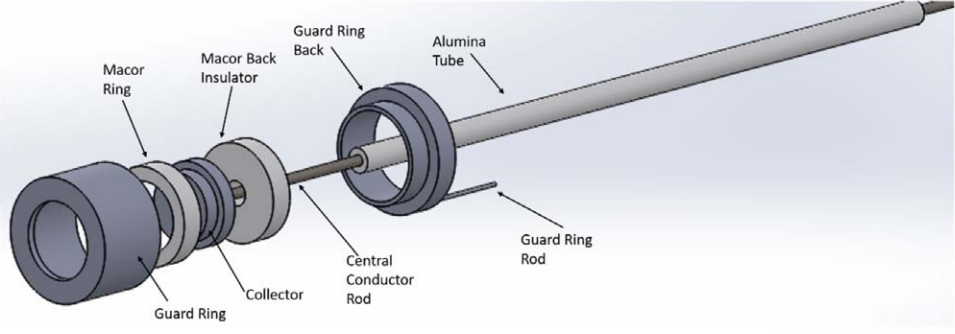
\includegraphics[width=\linewidth]{fig/faradayprobeexploded.png}
    \caption[Exploded view of guarded planar Faraday probe]{Exploded view of guarded planar Faraday probe\cite{yildiz2019plume}}
    \label{fig:explodedfaraday}
\end{figure}

\newpage

The probe is enclosed in a cylindirical conductive cylinder called guard ring and a collector plate is positioned at the base of the probe. Conductive ring and the collector is polarised with the same potential as shown in figure \ref{fig:faradayschematic} to ensure that the ion collection only occurs on the collector plate. 

\begin{figure}[ht]
    \centering
    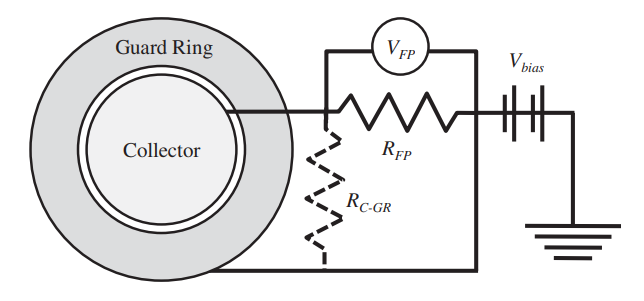
\includegraphics[scale=0.5]{fig/probeschematic.png}
    \caption[Working schematic of a guarded faraday probe]{Working schematic of a guarded faraday probe\cite{brown2017recommended}}
    \label{fig:faradayschematic}
\end{figure}


Probe would be positioned downstream of the ion beam and the opening of the probe would face the thruster so that the ions would enter the probe. Charge incurred on the collector plate would then be measured using a sourcemeter. This measurement would then be used to determine the amount of generated thrust. Faraday cup measurements would be performed in a hemispherical manner, as shown in figure \ref{fig:probepos}, which would also determine the beam divergence angle thus amount of lost thrust.

\begin{figure}[ht]
    \centering
    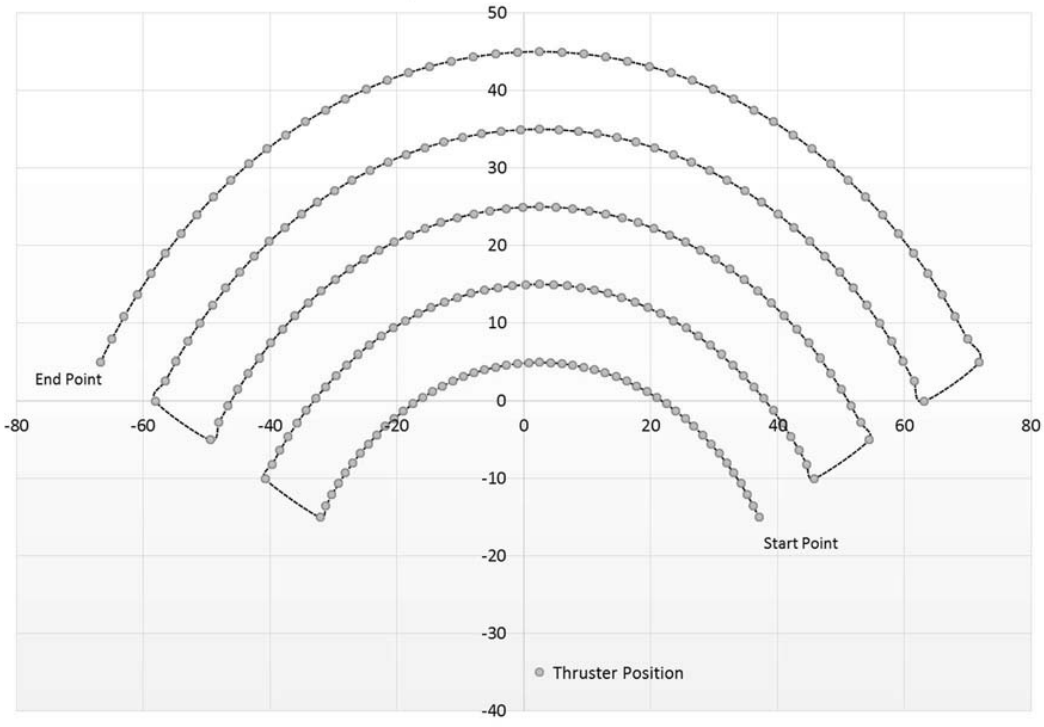
\includegraphics[scale=0.5]{fig/probepos.png}
    \caption[Faraday probe path and measurement points]{Faraday probe path and measurement points\cite{Couch2017}}
    \label{fig:probepos}
\end{figure}
\newpage

Another point for further study is to increase grid transparency in order to create more uniform ion beam out of created beamlets. This would increase the thrust generated by the ion thruster and also create a more visible ion beam. 

When the thruster was succesfully operated it was fitted with a grid with 61 apertures. Distance between apertures were 4.2 mm between each aperture. As future work thruster can be operated with a grid that has more closely located apertures. 

% \section{Practical Application of This Study}

% Lorem ipsum dolor sit amet, consetetur sadipscing elitr, sed diam nonumy eirmod tempor invidunt ut labore et dolore magna aliquyam erat, sed diam voluptua. At vero eos et accusam et justo duo dolores et ea rebum. Stet clita kasd gub rgren, no sea takimata sanctus est Lorem ipsum dolor sit amet, consetetur sadipscing elitr, sed diam nonumy eirmod tempor invidunt ut lab ore sit et dolore magna.

% \section{Second Level Title: First Letters Capital}


% \subsection{Third level title: Only first letter capital}

% \subsubsection{Fourth level title: Only first letter capital}


% This indicates that the ANN is accurate at base flow and flow height values lower then 3 m. 

% \begin{table*}[!htbp]
% 	{\setlength{\tabcolsep}{14pt}
% 		\caption{Example table in chapter 6.}
% 		\begin{center}
% 			\vspace{-6mm}
% 			\begin{tabular}{cccc}
% 				\hline \\[-2.45ex] \hline \\[-2.1ex]
% 				Column A & Column B & Column C & Column D \\
% 				\hline \\[-1.8ex]
% 				Row A & Row A & Row A & Row A \\
% 				Row B & Row B & Row B & Row B \\
% 				Row C & Row C & Row C & Row C \\
% 				[-0ex] \hline
% 			\end{tabular}
% 			\vspace{-6mm}
% 		\end{center}
% 		\label{Table6.1}}
% \end{table*}



% %{\bf Fifth level title: No numbering after fourth level titles}
% \subsubsubsection{Fifth level title: No numbering after fourth level titles}

% \begin{figure}
% 	\centering
% 	
\includegraphics[width=230pt,keepaspectratio=true]{./fig/sekil7}
% 	% sekil7.eps: 0x0 pixel, 300dpi, 0.00x0.00 cm, bb=14 14 455 369
% 	\caption{Example table in chapter 6.}
% 	\label{Figure6.1}
% \end{figure}



